\section{The Carrier-Roughness Useful-Memory Horizon Law}
\label{sec:finite_memory_under_drift}

Under drift, memory is both a statistical resource and a temporal liability.
Retaining more data reduces finite-sample noise, but it also increases the age
of the evidence used to represent the present. The object of interest is
therefore not a detector threshold or a particular adaptive rule, but the error
of finite-memory representation itself.

\begin{figure}[!htbp]
\centering
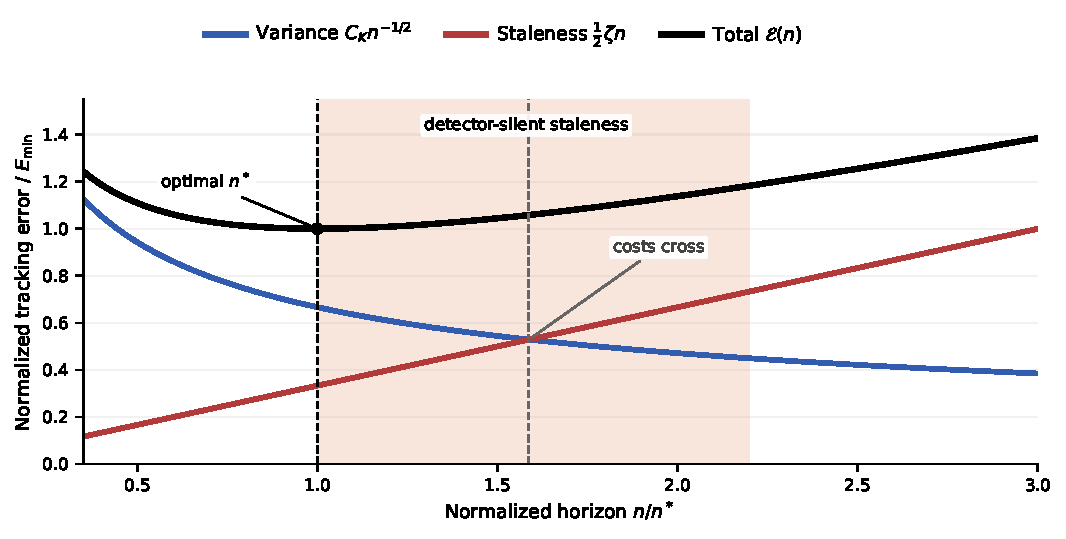
\includegraphics[width=0.92\linewidth]{artifacts/figures/conceptual/fig_two_clocks_of_drift.pdf}
\caption{Two clocks of drift. The finite-sample term falls with horizon, the
staleness term rises with age, and total error is minimized at the useful-memory
horizon $n^*$. The shaded region represents detector-silent staleness: retained
evidence can lose temporal validity before enough changepoint evidence
accumulates to trigger an alarm.}
\label{fig:two_clocks_of_drift}
\end{figure}

For a finite-memory estimator with lag weights $w_0,\dots,w_{n-1}$, the natural
age variable is the effective lag
\[
  A(w) \coloneqq \sum_{j=0}^{n-1} j\,w_j.
\]
Its corresponding staleness at time $t$ is the weighted transport misalignment
\[
  S_t(w) \coloneqq \sum_{j=0}^{n-1} w_j\,
  W_2\!\left(P_{t-j},P_t\right).
\]
For a uniform window, $A(w)=(n-1)/2$, so window length and temporal age are the
same object up to constants. This is why memory length becomes a statistical
question rather than a purely algorithmic one.

Throughout the paper, $P_t$ denotes the present target law,
$\bar P_t^{(n)}$ the window target obtained by averaging the last $n$ target
laws, and $\widehat P_t^{(n)}$ the estimator built from the last $n$
observations. The carrier term always refers to the estimation error relative to
$\bar P_t^{(n)}$, while the staleness term refers to the discrepancy between
$\bar P_t^{(n)}$ and $P_t$.

The theory repeatedly combines three ingredients: a carrier benchmark relative to
$\bar P_t^{(n)}$, a path-class control on the staleness between $\bar P_t^{(n)}$
and $P_t$, and, when available, a lower-bound or benchmark theorem showing that
the resulting horizon is structural on the geometry under study.

\subsection{Abstract Upper Law}\label{subsec:abstract_upper_law}

The abstract theorem separates finite-sample carrier behavior from
drift-induced staleness.

\begin{theorem}[Abstract upper law]\label{thm:abstract_upper_law}
Let $d$ be a probability metric satisfying the triangle inequality. At time $t$,
let $P_t$ be the present target law, let $\bar P_t^{(n)}$ be the window target,
and let $\widehat P_t^{(n)}$ be the estimator built from the last $n$
observations. Assume that for some constants $C_K>0$, $C_S>0$, exponent $a>0$,
roughness index $H\in(0,1]$, and amplitude $\zeta>0$,
\[
  \mathbb E\,d\!\left(\widehat P_t^{(n)},\bar P_t^{(n)}\right)
  \le C_K n^{-a}
\]
and
\[
  d\!\left(\bar P_t^{(n)},P_t\right)
  \le C_S\zeta n^H
\]
hold for all $n$ in the regime of interest. Then
\[
  \mathbb E\,d\!\left(\widehat P_t^{(n)},P_t\right)
  \le C_K n^{-a} + C_S\zeta n^H.
\]
\end{theorem}

\begin{proof}
By the triangle inequality,
\[
  d\!\left(\widehat P_t^{(n)},P_t\right)
  \le
  d\!\left(\widehat P_t^{(n)},\bar P_t^{(n)}\right)
  + d\!\left(\bar P_t^{(n)},P_t\right).
\]
Taking expectations and applying the two assumptions yields the claim.
\end{proof}

The proof is immediate, but the theorem makes the modular structure explicit:
the path class supplies the staleness term, while the chosen geometry and sample
regime supply the carrier term.

\begin{corollary}[Optimized useful-memory horizon law]
\label{cor:optimized_horizon}
Under the assumptions of \cref{thm:abstract_upper_law}, the upper envelope
\[
  \Phi(n) \coloneqq C_K n^{-a} + C_S\zeta n^H
\]
is minimized, up to constant factors, at
\[
  n^*(a,H) \asymp (C_K/\zeta)^{1/(a+H)},
\]
and the corresponding optimized error scale is
\[
  \Phi(n^*) \asymp C_K^{H/(a+H)}\zeta^{a/(a+H)}.
\]
\end{corollary}

\begin{proof}
Balance the decreasing carrier term against the increasing staleness term:
\[
  C_K n^{-a} \asymp C_S\zeta n^H.
\]
This gives $n^{a+H}\asymp C_K/\zeta$, hence the displayed horizon law. Substituting
that scale back into either term gives the optimized error scale.
\end{proof}

The cube-root law is recovered when $a=1/2$ and $H=1$. More generally, the
carrier exponent and the roughness exponent jointly determine the useful-memory
scale. There is no universal horizon independent of those two ingredients.

\subsection{Path Classes and the Roughness Index}

The staleness side of the law is controlled by a deterministic path class. For
$H\in(0,1]$ and $\zeta>0$, write
\[
  \mathfrak P_H(\zeta)
  \coloneqq
  \left\{(P_s)_{s\in\mathbb Z}: W_2(P_{t-j},P_t) \le \zeta j^H
  \text{ for all } j\ge 0\right\}.
\]
The case $H=1$ is the local Lipschitz envelope; smaller $H$ correspond to slower
accumulation of staleness with lag.

\begin{lemma}[Hölder staleness bound via averaged couplings]
\label{lem:Hölder_staleness_bound}
Let
\[
  \bar P_t^{(n)} \coloneqq \frac{1}{n}\sum_{j=0}^{n-1} P_{t-j}.
\]
If the target path belongs to $\mathfrak P_H(\zeta)$, then
\[
  W_2^2\!\left(\bar P_t^{(n)},P_t\right)
  \le
  \frac{\zeta^2}{n}\sum_{j=0}^{n-1} j^{2H},
\]
and therefore
\[
  W_2\!\left(\bar P_t^{(n)},P_t\right)
  \le \zeta\left(\frac{1}{n}\sum_{j=0}^{n-1} j^{2H}\right)^{1/2}
  = C_{H,n}\,\zeta n^H,
\]
where
\[
  C_{H,n}
  \coloneqq
  \left(n^{-(2H+1)}\sum_{j=0}^{n-1} j^{2H}\right)^{1/2}.
\]
In particular, $C_{H,n}\to (2H+1)^{-1/2}$ as $n\to\infty$.
\end{lemma}

\begin{proof}
For each lag $j$, let $\pi_j$ be an optimal coupling between $P_{t-j}$ and $P_t$.
Their average
\[
  \bar \pi \coloneqq \frac{1}{n}\sum_{j=0}^{n-1} \pi_j
\]
couples $\bar P_t^{(n)}$ with $P_t$, so
\[
  W_2^2\!\left(\bar P_t^{(n)},P_t\right)
  \le
  \int \|x-y\|^2\,d\bar\pi(x,y)
  =
  \frac{1}{n}\sum_{j=0}^{n-1} W_2^2\!\left(P_{t-j},P_t\right).
\]
Applying the Hölder envelope gives the displayed finite-$n$ constant, and taking
square roots completes the proof.
\end{proof}

Combining \cref{lem:Hölder_staleness_bound} with
\cref{cor:optimized_horizon} yields the family
\[
  n^*(a,H) \asymp (C_K/\zeta)^{1/(a+H)}.
\]
On the canonical statistical regime $a=1/2$,
\[
  n^*(1/2,H) \asymp (C_K/\zeta)^{2/(1+2H)}.
\]
At $H=1$, this recovers the cube-root horizon; at $H=1/2$, it yields the
intermediate $n^*\asymp C_K/\zeta$ regime. These are members of the same law,
not separate theorem stories. The finite-$n$ constant in
\cref{lem:Hölder_staleness_bound} is the constant used throughout the paper for
uniform windows; the simpler $(2H+1)^{-1/2}$ expression is its large-window
limit.

\subsection{Minimum Kernel: A Rigorous Carrier Instantiation}
\label{subsec:minimum_kernel}

The abstract law needs at least one rigorous carrier instantiation. The minimum
kernel is the bounded-support fixed-span one-dimensional triangular array. It
provides the first rigorous carrier entering the abstract horizon law.

\begin{proposition}[Minimum-kernel carrier]\label{prop:minimum_kernel}
Let $X_{n,1},\dots,X_{n,n}$ be independent one-dimensional observations with laws
$P_{n,1},\dots,P_{n,n}$, and define the window mixture
\[
  \bar P_n = \frac{1}{n}\sum_{j=1}^n P_{n,j}.
\]
Assume:
\begin{enumerate}[label=(\roman*)]
  \item all $P_{n,j}$ are supported on a common compact interval $[L,U]$;
  \item the within-window drift span is uniformly bounded in $n$;
  \item on an interior quantile band $u\in[\varepsilon,1-\varepsilon]$, the mixture
  density $\bar f_n$ is bounded below and uniformly Hölder;
  \item the triangular-array empirical quantile process admits a Bahadur
  representation with integrated remainder $o(n^{-1})$ on that interior band.
\end{enumerate}
Then
\[
  \mathbb E\,W_2^2\!\left(\widehat P_n^{\mathrm{tri}},\bar P_n\right)=O(n^{-1}),
\]
and therefore
\[
  \mathbb E\,W_2\!\left(\widehat P_n^{\mathrm{tri}},\bar P_n\right)=O(n^{-1/2}).
\]
\end{proposition}

\paragraph{Proof sketch.}
In one dimension,
\[
  W_2^2\!\left(\widehat P_n^{\mathrm{tri}},\bar P_n\right)
  = \int_0^1 \bigl(\widehat q_n(u)-q_n(u)\bigr)^2\,du,
\]
so the problem reduces to the integrated $L_2$ error of the empirical quantile
process. On the interior band, the Bahadur representation gives
\[
  \widehat q_n(u)-q_n(u)
  =
  \frac{u-\widehat F_n(q_n(u))}{\bar f_n(q_n(u))} + R_n(u).
\]
The leading term has integrated variance $O(n^{-1})$ because the observations are
independent and the fixed-span triangular design changes only constants relative
to the i.i.d. mixture benchmark. The remainder splits into an empirical
increment term and a Taylor term; the empirical increment term is the dominant
one, but under the stated interior regularity it still satisfies an integrated
$o(n^{-1})$ bound. Bounded support makes the boundary-band contribution
lower-order. Summing the leading term, the lower-order cross term, and the
integrated remainder gives $\mathbb E W_2^2=O(n^{-1})$, and Jensen yields the
displayed $W_2$ rate.

The main conclusion is the exponent. Under this bounded-support fixed-span
regime, the triangular-array carrier remains root-$n$ and differs from the
i.i.d. mixture benchmark only through a design effect.

\begin{remark}[A self-contained sufficient package]
The nonstandard assumption in \cref{prop:minimum_kernel} is item~(iv). A
practical sufficient package for the regime intended here is the following:
independence across the row, common bounded support, uniformly bounded
within-window span, mixture quantiles that stay on an interior band where
$\bar f_n$ is bounded below and uniformly H\"older, and row-wise perturbations of
the i.i.d. mixture benchmark that change the empirical-process variance only by a
fixed-span design effect. In that setting, the usual one-dimensional Bahadur
expansion for smooth quantile functionals yields an integrated remainder
$o(n^{-1})$. This covers, for example, bounded-support smooth location
perturbations of a common base density and bounded smooth monotone transforms of
such a base law, provided the fixed-span condition is maintained.
\end{remark}

\subsection{A Structural Lower Bound}\label{subsec:lower_bound}

The upper law would be substantially weaker if it were only the optimum of one
estimator. The lower bound shows that, on the canonical carrier regime $a=1/2$,
the useful-memory scale is imposed by the drift geometry itself.

\begin{figure}[!htbp]
\centering
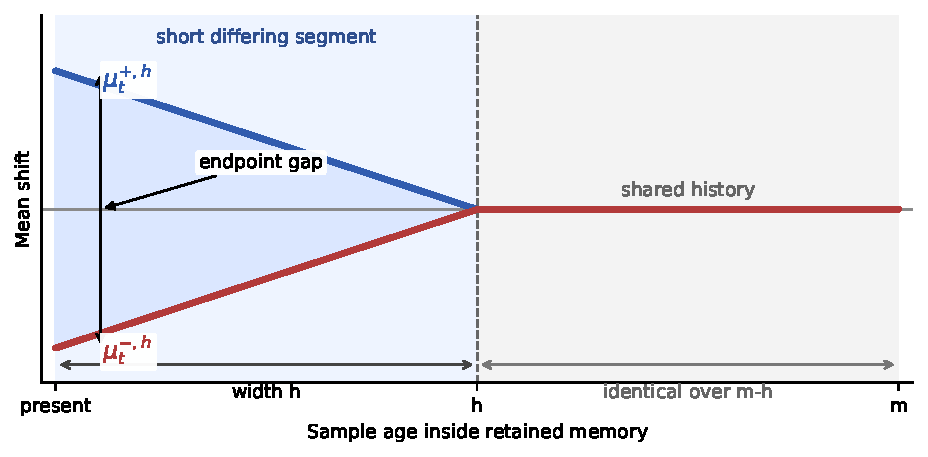
\includegraphics[width=0.88\linewidth]{artifacts/figures/conceptual/fig_lower_bound_witness.pdf}
\caption{Gaussian witness for the structural lower bound. The two paths share
most of the retained history and differ only on a recent segment of width $h$,
yet remain separated at the present. Optimizing that recent segment already
produces the same horizon exponent as the upper law on the canonical carrier
regime.}
\label{fig:lower_bound_witness}
\end{figure}

\begin{proposition}[Structural lower bound on the canonical carrier regime]
\label{prop:structural_lower_bound}
Fix $H\in(0,1]$ and work on the Gaussian location subclass with known variance
$\sigma^2$ and witness paths
\[
  \mu_{t-j}^{\pm,h} = \pm \beta (h-j)_+^H,
  \qquad j=0,1,\dots,h,
\]
where $\beta\le \zeta$ enforces the roughness budget. Let
\(\mathcal G_{H,\zeta}^{\mathrm{Gauss}}\) denote the corresponding Gaussian
location subclass of target paths. Then there exists a
constant $c_H>0$ depending only on $H$ such that the endpoint tracking risk over
this subclass satisfies
\[
  \inf_{\widehat P}\sup_{P\in\mathcal G_{H,\zeta}^{\mathrm{Gauss}}}
  \mathbb E\,W_2\!\left(\widehat P_t,P_t\right)
  \ge c_H\,\sigma^{2H/(2H+1)}\zeta^{1/(2H+1)}.
\]
Consequently, on the canonical carrier regime $a=1/2$, the useful-memory scale
\[
  h^*(H) \asymp (\sigma/\zeta)^{2/(2H+1)}
\]
is structural even on this restricted subclass.
\end{proposition}

\paragraph{Proof sketch.}
Compare two hypotheses generated by the witness paths
$\mu_{t-j}^{+,h}$ and $\mu_{t-j}^{-,h}$. At the present time, the endpoint
separation is of order $\beta h^H$. On the Gaussian location subclass, this is
also the $W_2$ separation. The Kullback--Leibler divergence between the two
hypotheses is proportional to
\[
  \beta^2 \sum_{r=1}^h r^{2H}/\sigma^2.
\]
Choosing
\[
  \beta = \min\!\left\{\zeta,\frac{\sigma}{2\sqrt{\sum_{r=1}^h r^{2H}}}\right\}
\]
keeps the testing problem in the Le Cam regime while respecting the roughness
budget. The resulting two-point lower bound is of order $\beta h^H$. Balancing
the active roughness constraint against the testing constraint gives
$h^*(H)\asymp (\sigma/\zeta)^{2/(2H+1)}$ and therefore the displayed lower law.

At $H=1$, this recovers the cube-root horizon and the lower scale
$\sigma^{2/3}\zeta^{1/3}$. The lower bound is subclass based rather than
class-tight, but that is enough for the central claim: the horizon is
not just an estimator artifact.

The proposition above is the lower-bound fact needed for the main horizon law.
The same witness analysis also exposes a sharper constant-level geometry. We
record those refinements next because they explain what is intrinsic to the
canonical $a=1/2$ regime and what was only an artifact of the original ramp proof
with its testing relaxation.

\subsection{Refined Geometry of the Gaussian Witness}
\label{subsec:refined_witness_geometry}

Let $\Phi$ and $\varphi$ denote the standard normal distribution function and
density.
For the ramp witness in \cref{prop:structural_lower_bound}, exact Gaussian
testing gives a one-dimensional variational problem rather than a Pinsker-style
constant.

\begin{proposition}[Exact Gaussian ramp frontier]
\label{prop:exact_gaussian_ramp_frontier}
Fix $H\in(0,1]$ and set
\[
  p_H \coloneqq \frac{2H}{2H+1}.
\]
Let $x_H>0$ be the unique maximizer of $x^{p_H}\Phi(-x)$, equivalently the
solution of
\[
  p_H\Phi(-x_H)=x_H\varphi(x_H).
\]
For the Gaussian ramp witness
\[
  \mu_{t-j}^{\pm,h}=\pm\beta(h-j)_+^H,
\]
the exact two-point lower bound has asymptotic constant
\[
  C_H^{\mathrm{ramp}}
  =
  (2H+1)^{H/(2H+1)}x_H^{2H/(2H+1)}\Phi(-x_H),
\]
with horizon shape
\[
  h_H^*\sim
  (\sqrt{2H+1}\,x_H)^{2/(2H+1)}
  \left(\frac{\sigma}{\zeta}\right)^{2/(2H+1)}.
\]
\end{proposition}

\begin{proof}[Proof sketch]
For fixed $h$, the likelihood-ratio testing problem between the two Gaussian
paths depends on
\[
  S_h=\sum_{r=1}^h r^{2H}
\]
and has exact Bayes error $\Phi(-\beta\sqrt{S_h}/\sigma)$. The endpoint loss is
of order $\beta h^H$, so the witness objective is
\[
  L_h(\beta)=\beta h^H\Phi(-\beta\sqrt{S_h}/\sigma).
\]
In the large-ratio regime $\sigma/\zeta\to\infty$, use
$S_h\sim h^{2H+1}/(2H+1)$ and set
$x=\zeta\sqrt{S_h}/\sigma$. After normalizing by
$\sigma^{2H/(2H+1)}\zeta^{1/(2H+1)}$, the objective becomes
$(2H+1)^{H/(2H+1)}x^{p_H}\Phi(-x)$. Differentiating gives the stated scalar
equation and constant.
\end{proof}

The ramp is therefore a valid structural witness, but it is not the best
endpoint-saturating H\"older shape when $H<1$.

\begin{proposition}[Endpoint-minimal witness as the energy minimizer]
\label{prop:endpoint_minimal_witness}
Fix $H\in(0,1]$ and $h\ge 1$. Among all discrete profiles
$g=(g_0,\dots,g_h)$ satisfying
\[
  g_0=0,
  \qquad
  g_h=h^H,
  \qquad
  |g_r-g_s|\le |r-s|^H,
\]
the profile
\[
  g_r^{\min}=h^H-(h-r)^H
\]
minimizes the testing energy $\sum_{r=1}^h g_r^2$. Its asymptotic energy constant is
\[
  I_H
  =
  \int_0^1 \left(1-(1-u)^H\right)^2du
  =
  \frac{2H^2}{(H+1)(2H+1)}.
\]
Consequently the exact Gaussian endpoint-minimal witness has constant
\[
  C_H^{\min}
  =
  I_H^{-H/(2H+1)}x_H^{2H/(2H+1)}\Phi(-x_H),
\]
where $x_H$ is the root from \cref{prop:exact_gaussian_ramp_frontier}. For
$H<1$, this strictly improves the ramp constant by the factor
\[
  \left(\frac{H+1}{2H^2}\right)^{H/(2H+1)}.
\]
\end{proposition}

\begin{proof}
For any feasible profile, the endpoint constraint and H\"older condition imply
\[
  g_r\ge h^H-(h-r)^H.
\]
The displayed $g^{\min}$ attains this lower envelope and is feasible because
$x\mapsto x^H$ is subadditive on $(0,\infty)$ for $H\le 1$. It is therefore
pointwise dominated by every feasible profile and minimizes
$\sum_{r=1}^h g_r^2$. The Riemann-sum limit gives
\[
  h^{-(2H+1)}\sum_{r=1}^h \left(h^H-(h-r)^H\right)^2\to I_H.
\]
Substituting a general energy constant $I$ into the exact Gaussian reduction gives
$I^{-H/(2H+1)}x_H^{2H/(2H+1)}\Phi(-x_H)$. Taking
$I=I_H$ yields the endpoint-minimal constant; comparing it with the ramp energy
constant $(2H+1)^{-1}$ gives the improvement factor. At $H=1$, the two profiles
coincide.
\end{proof}

These refinements matter for more than witness design. They also change the
constant-level interpretation of the canonical lower regime. Once the roughness
side is expressed through the exact uniform-window staleness constant and the
lower side uses the exact Gaussian witness constants, the remaining proof gap has
a clean structural form.

\begin{proposition}[Refined proof-gap consequence on the canonical witness regime]
\label{prop:refined_proof_gap}
Fix $H\in(0,1]$ and let
\[
  C_S^{\mathrm{asymp}}(H) \coloneqq (2H+1)^{-1/2}.
\]
For $a>0$, define
\[
  \Sigma(a,H)
  \coloneqq
  \left(\frac{a}{a+H}\right)^{-a/(a+H)}
  +
  \left(\frac{H}{a+H}\right)^{-H/(a+H)}.
\]
For either refined witness constant
\[
  C_H^{\mathrm{ref}}\in\{C_H^{\mathrm{ramp}},C_H^{\min}\},
\]
consider the associated constant-level proof-gap formula
\[
  \Gamma_{\mathrm{ref}}(a,H)
  =
  \Sigma(a,H)
  \left(\frac{C_S^{\mathrm{asymp}}(H)}{C_H^{\mathrm{ref}}}\right)^{a/(a+H)}.
\]
Then, for every fixed $H\in(0,1]$,
\[
  \inf_{a>0}\Gamma_{\mathrm{ramp}}(a,H)
  =
  \inf_{a>0}\Gamma_{\min}(a,H)
  =2,
\]
and the infimum is attained only in the boundary limit $a\downarrow 0$.
\end{proposition}

\begin{proof}[Proof sketch]
Write
\[
  p=\frac{2H}{2H+1}\in(0,2/3].
\]
For the ramp witness, the scalar root equation
\[
  p\Phi(-x_H)=x_H\varphi(x_H)
\]
together with the Komatsu-style bound
\[
  \Phi(-x)
  \le
  \frac{2\varphi(x)}{x+\sqrt{x^2+8/\pi}}
\]
gives the explicit lower envelope
\[
  \frac{C_S^{\mathrm{asymp}}(H)}{C_H^{\mathrm{ramp}}}
  \ge
  \sqrt{2\pi}
  \frac{(1-p)^{(p+1)/2}(p+2/\pi)^{(p+1)/2}}{p^p}.
\]
Splitting at $p_0=1-2/\pi$ (equivalently $H_0=\pi/4-1/2$) reduces this lower
envelope to two elementary log-concave functions whose endpoint values are all
strictly larger than $1$. Hence
\[
  C_S^{\mathrm{asymp}}(H)>C_H^{\mathrm{ramp}}
  \qquad\text{for all }H\in(0,1].
\]

For the endpoint-minimal witness, the same tail bound gives
\[
  \frac{C_S^{\mathrm{asymp}}(H)}{C_H^{\min}}
  \ge
  \sqrt{2\pi}\,\sqrt{1-p}
  \frac{(p+2/\pi)^{(p+1)/2}}{(2-p)^{p/2}}.
\]
The logarithmic derivative of this lower envelope admits an explicit upper bound
whose numerator is a cubic polynomial in $p$ with negative derivative on
$p\in(0,2/3]$. The lower envelope is therefore strictly decreasing, so its
minimum is forced to the endpoint $p=2/3$, where it is still strictly larger
than $1$. Hence
\[
  C_S^{\mathrm{asymp}}(H)>C_H^{\min}
  \qquad\text{for all }H\in(0,1].
\]

For either refined constant, set
\[
  R_{\mathrm{ref}}(H)=C_S^{\mathrm{asymp}}(H)/C_H^{\mathrm{ref}}>1.
\]
Then
\[
  \Gamma_{\mathrm{ref}}(a,H)=\Sigma(a,H)R_{\mathrm{ref}}(H)^{a/(a+H)}.
\]
Since $\Sigma(a,H)\ge 2$ and $R_{\mathrm{ref}}(H)^{a/(a+H)}\ge 1$, one has
$\Gamma_{\mathrm{ref}}(a,H)\ge 2$. As $a\downarrow 0$, the exponent
$a/(a+H)\downarrow 0$ and $\Sigma(a,H)\to 2$, so
$\Gamma_{\mathrm{ref}}(a,H)\to 2$. This yields the displayed infimum formula.
\end{proof}

This proposition has the same scope as the refined witness geometry itself. It
does not claim a class-tight minimax theorem for all deterministic H\"older
paths. Its role is narrower and cleaner: within the exact
Gaussian witness program, the conservative constant from the older testing
relaxation is replaced by witness-level constants for which the residual gap is
exactly the structural factor-two crossover between additive upper and two-point
lower mechanisms.

The same refined witness geometry also yields a full class-level benchmark once
the model is specialized to Gaussian location tracking. In that setting, the
deterministic H\"older envelope, the finite-memory estimator, and the lower-bound
witness all live in the same one-dimensional parameterization, so the canonical
regime admits a direct minimax rate statement.

\begin{theorem}[Gaussian location minimax benchmark on the deterministic H\"older class]
\label{thm:gaussian_location_minimax_holder}
Fix $H\in(0,1]$, $\zeta>0$, and $\sigma>0$. Let $\mathfrak M_H(\zeta)$ denote the
class of deterministic mean paths $(\mu_s)_{s\in\mathbb Z}$ such that
\[
  |\mu_{t-j}-\mu_t|\le \zeta j^H
  \qquad\text{for all }j\ge 0.
\]
Suppose the observations are independent with
\[
  Y_{t-j}\sim N(\mu_{t-j},\sigma^2),
  \qquad j=0,1,\dots,n-1,
\]
and let the target law at time $t$ be $P_t=N(\mu_t,\sigma^2)$. Define the
optimized finite-memory minimax risk
\[
  \mathcal R_H^*(\sigma,\zeta)
  \coloneqq
  \inf_{n\ge 1}
  \inf_{\widehat P_t^{(n)}}
  \sup_{\mu\in\mathfrak M_H(\zeta)}
  \mathbb E\,W_2\!\left(\widehat P_t^{(n)},P_t\right).
\]
Then there exist constants $0<c_H\le C_H<\infty$, depending only on $H$, such that
\[
  c_H\,\sigma^{2H/(2H+1)}\zeta^{1/(2H+1)}
  \le
  \mathcal R_H^*(\sigma,\zeta)
  \le
  C_H\,\sigma^{2H/(2H+1)}\zeta^{1/(2H+1)}.
\]
In particular, the deterministic H\"older class has the canonical minimax horizon
scale
\[
  n_H^*\asymp (\sigma/\zeta)^{2/(2H+1)}.
\]
Moreover, the uniform-window mean estimator has an exact asymptotic upper
constant on this benchmark. If $y_H>0$ solves
\[
  H y_H\bigl(2\Phi(y_H)-1\bigr)=\varphi(y_H),
\]
then its asymptotic horizon shape is
\[
  A_H^{\mathrm{mean}}=((H+1)y_H)^{2/(2H+1)}
\]
and its asymptotic risk constant is
\[
  U_H^{\mathrm{mean}}
  =
  ((H+1)y_H)^{-1/(2H+1)}
  \Bigl(2\varphi(y_H)+y_H\bigl(2\Phi(y_H)-1\bigr)\Bigr).
\]
\end{theorem}

\begin{proof}[Proof sketch]
For the upper bound, estimate the present mean by the uniform-window average
\[
  \widehat\mu_t^{(n)}\coloneqq \frac{1}{n}\sum_{j=0}^{n-1}Y_{t-j}
\]
and set $\widehat P_t^{(n)}=N(\widehat\mu_t^{(n)},\sigma^2)$. Because equal-variance
Gaussian laws satisfy
\[
  W_2\!\left(N(m_1,\sigma^2),N(m_2,\sigma^2)\right)=|m_1-m_2|,
\]
the risk reduces to mean estimation error. The noise term is
$\sigma\sqrt{2/(\pi n)}$, while the deterministic bias is bounded by
\[
  \frac{\zeta}{n}\sum_{j=0}^{n-1} j^H,
\]
so
\[
  \sup_{\mu\in\mathfrak M_H(\zeta)}
  \mathbb E\,W_2\!\left(\widehat P_t^{(n)},P_t\right)
  \le
  \sigma\sqrt{\frac{2}{\pi n}} + \frac{\zeta}{n}\sum_{j=0}^{n-1} j^H.
\]
Rescaling by $n=A(\sigma/\zeta)^{2/(2H+1)}$ yields a one-parameter normalized
upper envelope. Differentiating its exact Gaussian-location form gives the stated
root equation for $y_H$, and therefore the displayed asymptotic upper constant
and horizon shape. In particular, this proves the stated upper rate and horizon
scale.

For the lower bound, use the symmetric two-point subfamily
\[
  \mu_{t-j}^{\pm,h}=\pm \beta\bigl(h^H-j^H\bigr)_+,
  \qquad j\ge 0,
\]
with $\beta\le \zeta$. This family lies in $\mathfrak M_H(\zeta)$ because
\[
  |\mu_t^{\pm,h}-\mu_{t-j}^{\pm,h}|=\beta\min(h^H,j^H)\le \zeta j^H.
\]
Moreover, for fixed endpoint value $\beta h^H$, it minimizes the Gaussian testing
energy over all symmetric lag profiles allowed by the present-point H\"older
envelope, since each lag coordinate is independently minimized by
$\beta(h^H-j^H)_+$. The exact Gaussian two-point calculation from the refined
witness analysis therefore applies on the full deterministic H\"older class and
yields a lower bound of order
\[
  \sigma^{2H/(2H+1)}\zeta^{1/(2H+1)}.
\]
Optimizing over $h$ gives the same horizon scale $(\sigma/\zeta)^{2/(2H+1)}$.
Combining the two sides proves the theorem.
\end{proof}

\subsection{Beyond the Minimum Kernel}

The one-dimensional minimum kernel is the first rigorous carrier instantiation.
Two broader settings are also important for interpreting the law.

\paragraph{Extended regime.}
In low-dimensional or low-intrinsic-dimensional settings, the natural question
is whether the triangular-array carrier inherits the same exponent as the i.i.d.
mixture benchmark up to a constant-level gap. The clearest evidence comes from
embedded $k=1$ support inside a larger ambient space, where triangular and
i.i.d. slopes remain near the $a=1/2$ regime under fixed span.

\paragraph{Operational regime.}
For a practical geometry such as fixed-$\varepsilon$ debiased Sinkhorn, the
corresponding question is whether the induced finite-sample carrier is stable
enough to enter the same horizon law. The experiments reported below support
that interpretation: on embedded low-intrinsic-dimensional support, the
triangular and i.i.d. benchmark carriers remain close across the tested
regularization values, with $\varepsilon$ affecting constants more than the
qualitative carrier exponent. The relevant theorem in this regime therefore does
not take the form of a raw-$W_2$ statement in arbitrary dimension, but of an
operational carrier theorem of
the form
\[
  \mathbb E\,S_{\varepsilon}\!\left(\widehat P_{t,\mathrm{tri}}^{(n)},\bar P_t^{(n)}\right)
  \le C_{\varepsilon} n^{-a_{\varepsilon}}
\]
under bounded support, fixed span, and structural low-dimensionality, where
$S_{\varepsilon}$ denotes a fixed-$\varepsilon$ Sinkhorn-type geometry and the
exponent $a_{\varepsilon}$ matches the corresponding i.i.d. mixture benchmark.
For fixed-$\varepsilon$ entropic transport quantities, theorem-level i.i.d.
results already point in this direction. Stromme proves minimum-intrinsic-
dimension scaling for Sinkhorn divergence values under bounded Lipschitz costs,
with the statistical error governed by the smaller covering complexity of the two
measures \citep[Theorem~3.1]{Stromme2023MID}. Groppe and Hundrieser prove lower-
complexity adaptation for empirical entropic OT costs and show that the finite-
iteration Sinkhorn algorithm preserves the same statistical order up to an
explicit computational tolerance \citep[Theorem~4.10 and
Remark~4.11]{GroppeHundrieser2024LCA}. On the embedded fixed-span model studied
here, the remaining structural pieces can also be isolated cleanly: the
triangular-window and i.i.d.-mixture supports have identical axis-aligned
covering complexity at operational scale, and with squared-Euclidean cost the
dual smoothness condition reduces to the LCA threshold $\alpha>k/2$. This makes
the operational question structurally sharp rather than amorphous: once the
triangular-vs.-i.i.d. carrier gap is calibrated on a regularization band, the
horizon law can be stated on that certified region.

\begin{definition}[Certified operational region]
\label{def:certified_operational_region}
Fix a bounded embedded fixed-span model, an intrinsic complexity index $k$, a
dual H\"older smoothness level $\alpha$, and an operational band
$\mathcal B\subset(0,\infty)$ of regularization values. We call
$(k,\mathcal B)$ a certified operational region for fixed-$\varepsilon$
Sinkhorn if:
\begin{enumerate}[label=(\roman*)]
  \item the i.i.d. fixed-$\varepsilon$ benchmark on the same support class
  admits a carrier bound with exponent $a_{\varepsilon}$ on $\mathcal B$;
  \item the triangular-window and i.i.d.-mixture supports have identical
  operational covering complexity on $\mathcal B$;
  \item the dual class lies in the parametric adaptation region $\alpha>k/2$;
  \item across $\mathcal B$, the calibrated triangular and i.i.d. carrier slopes
  stay useful and uniformly close.
\end{enumerate}
\end{definition}

\begin{proposition}[Certified operational frontier]
\label{prop:operational_theorem_frontier}
On the bounded embedded fixed-span model with squared-Euclidean cost, the first
three items in \cref{def:certified_operational_region} are structural: the
support-complexity inheritance is exact, and the dual-complexity condition is
precisely the LCA threshold $\alpha>k/2$. Consequently, any calibrated band
$\mathcal B$ satisfying item~(iv) supports the carrier-roughness horizon law on
a certified operational region. In particular, on bands where the i.i.d.
benchmark stays in the parametric Sinkhorn regime, the operational carrier takes
the canonical form
\[
  \mathbb E\,S_{\varepsilon}\!\left(\widehat P_{t,\mathrm{tri}}^{(n)},\bar P_t^{(n)}\right)
  \le C_{\varepsilon} n^{-1/2},
  \qquad \varepsilon\in\mathcal B,
\]
and the corresponding useful-memory scale is
\[
  n_{\varepsilon}^*(H) \asymp (C_{\varepsilon}/\zeta)^{1/(H+1/2)}.
\]
More generally, if the i.i.d. benchmark on $\mathcal B$ has exponent
$a_{\varepsilon}$, then the operational horizon law on that region is
\[
  n_{\varepsilon}^*(a_{\varepsilon},H)
  \asymp (C_{\varepsilon}/\zeta)^{1/(a_{\varepsilon}+H)}.
\]
\end{proposition}

\paragraph{Proof sketch.}
The i.i.d. side is the benchmark supplied by
\citet{Stromme2023MID} and \citet{GroppeHundrieser2024LCA}. In the present
embedded fixed-span model, the triangular-window and i.i.d.-mixture supports
have identical operational covering bounds, so the support-complexity side of
the inheritance problem is already closed. The squared-Euclidean chart model is
smooth enough that the dual-complexity condition reduces to $\alpha>k/2$, which
is exactly the parametric LCA region. Once the triangular-vs.-i.i.d. carrier gap
is calibrated to remain uniformly small on $\mathcal B$, the operational carrier
enters the abstract upper law just like any other carrier exponent. Optimizing
the resulting upper envelope gives the displayed horizon scale.

This proposition isolates the structural part of the operational story and the
point at which calibration still enters. It does not yet prove a full
triangular-array Sinkhorn theorem with explicit uniform constants across
$\mathcal B$; rather, it identifies a certified region in which the abstract
horizon law is justified by a closed i.i.d. benchmark, an exact complexity
inheritance statement, and a calibrated triangular-vs.-benchmark comparison.

\begin{corollary}[Certified fixed-$\varepsilon$ operational region]
\label{cor:certified_operational_region}
In the synthetic embedded fixed-span calibration used in this paper, with
$\alpha=2$ and span $0.25$, the maximal certified regularization
bands are:
\[
  \varepsilon_{\max}=0.5 \text{ for } (d,k)\in\{(8,1),(8,2),(12,2)\},
  \qquad
  \varepsilon_{\max}=0.2 \text{ for } (d,k)=(12,1).
\]
Thus the operational frontier is not a dimension-free blanket statement. It is a
certified region inside the fixed-span model on which the practical Sinkhorn
carrier inherits the useful-memory law of the corresponding i.i.d. benchmark.
\end{corollary}

\begin{figure}[!htbp]
\centering
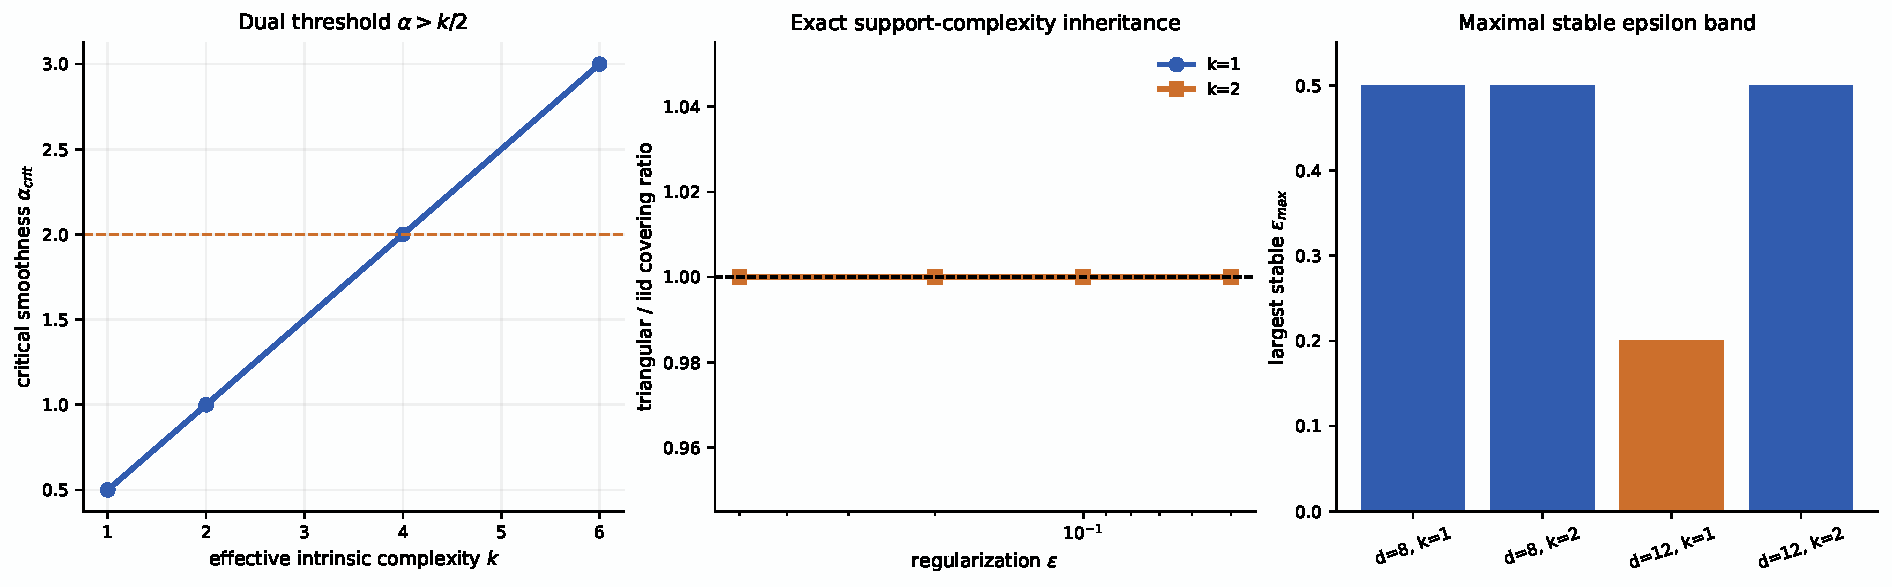
\includegraphics[width=0.94\linewidth]{artifacts/figures/frontier/fig_operational_theorem_mechanism.pdf}
\caption{Certified operational frontier. Left: the dual threshold
$\alpha>k/2$ that identifies the parametric adaptation regime. Middle: exact
support-complexity inheritance in the embedded fixed-span model. Right: maximal
certified $\varepsilon$-bands in the calibrated synthetic setting. Together these
three ingredients isolate the operational region on which fixed-$\varepsilon$
Sinkhorn supports the same carrier-roughness horizon law as its i.i.d.
benchmark.}
\label{fig:operational_theorem_mechanism}
\end{figure}

\paragraph{Regular-family extension target.}
The noncanonical question is broader than preserving the root-$n$ carrier. The
relevant objective is to identify distribution families and geometries that
support some member of the carrier-roughness horizon family, with carrier exponent
$a=a(\mathcal G)$ determined by the geometry rather than fixed a priori. A
natural candidate class is a locally regular dominated family: a parameterized
family $\{P_\theta: \theta\in\Theta\}$ with a
common dominating measure, locally quadratic testing geometry,
\[
  \KL(P_\theta,P_{\theta'})\asymp \|\theta-\theta'\|^2,
\]
and local comparability between parameter displacement and the chosen metric,
\[
  d(P_\theta,P_{\theta'})\asymp \|\theta-\theta'\|^{\alpha}
\]
for some metric exponent $\alpha>0$. In such a family, a deterministic H\"older
envelope in parameter space transfers to a deterministic staleness law in the
observation geometry with metric roughness exponent $\alpha H$, while the i.i.d.
carrier problem remains regular enough for Le Cam-style lower arguments and
benchmark upper laws to interact on a common local scale.

\begin{conjecture}[Regular-family horizon inheritance]
\label{conj:regular_family_horizon_inheritance}
Let $d$ be a probability geometry and let $\{P_\theta: \theta\in\Theta\}$ be a
locally regular dominated family for which the i.i.d. benchmark satisfies a
metric carrier law
\[
  \mathbb E\,d\!\left(\widehat P_{\mathrm{iid}}^{(n)},P_\theta\right)
  \le C_K n^{-a}
\]
uniformly on the parameter region of interest. Suppose the path obeys a
deterministic H\"older envelope in parameter space,
\[
  \|\theta_{t-j}-\theta_t\|\le \zeta j^H.
\]
Then the induced metric staleness should scale as
\[
  d(P_{\theta_{t-j}},P_{\theta_t})\lesssim \zeta^{\alpha}j^{\alpha H},
\]
so the corresponding tracking problem should satisfy the horizon-family member
\[
  n^*(a,\alpha H)\asymp (C_K/\zeta^{\alpha})^{1/(a+\alpha H)},
\]
with optimized risk of order
\[
  C_K^{\alpha H/(a+\alpha H)}\zeta^{\alpha a/(a+\alpha H)}.
\]
In the locally regular parametric subcase, the natural metric carrier exponent is
$a=\alpha/2$, giving the horizon scale
\[
  n^*(\alpha/2,\alpha H)
  \asymp (C_K/\zeta^{\alpha})^{1/(\alpha(1/2+H))}.
\]
\end{conjecture}

\begin{figure}[!htbp]
\centering
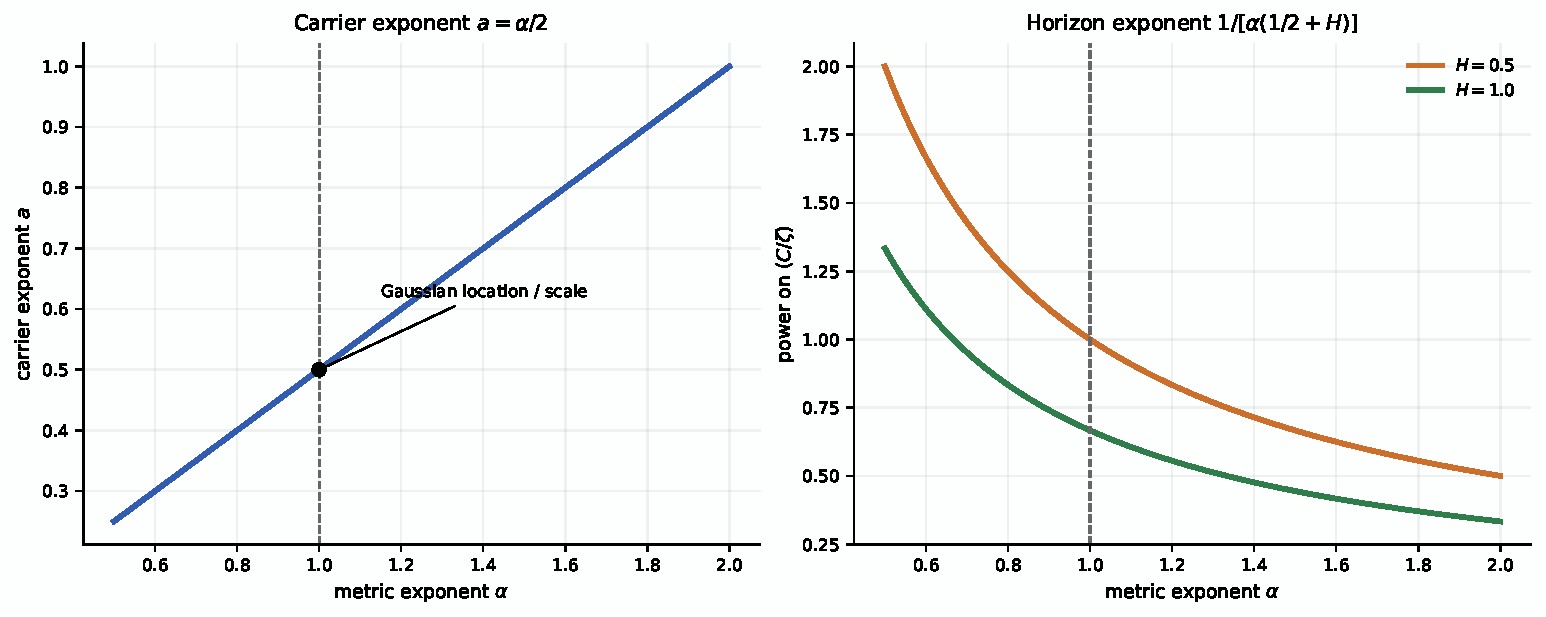
\includegraphics[width=0.92\linewidth]{artifacts/figures/frontier/fig_regular_family_inheritance.pdf}
\caption{Regular-family inheritance beyond the canonical case. Left: if the
metric geometry scales as $d(P_\theta,P_{\theta'})\asymp
\|\theta-\theta'\|^{\alpha}$, then the natural parametric metric carrier is
$a=\alpha/2$. Right: the resulting horizon exponent becomes
$1/[\alpha(1/2+H)]$, so the canonical Gaussian-location/Gaussian-scale regime
appears as the distinguished slice $\alpha=1$ rather than as a universal rule.}
\label{fig:regular_family_inheritance}
\end{figure}

This figure makes the noncanonical point concrete. The right extension problem
is not to preserve the canonical horizon law for every family, but to identify
which family geometry induces which carrier exponent and therefore which member
of the horizon family.

The distinction between regular, support-changing, and singular families shows
why such a regularity package is necessary.
Continuous one-dimensional scale families such as Gaussian scale and uniform
scale are broadly compatible with the same horizon exponent, but their local
testing geometry differs sharply: Gaussian scale is regular, whereas uniform
scale has support-driven nonregularity and atomic scale families become singular.
So a full distributional extension should be formulated for regular dominated
families or operational geometries with comparable local behavior, not for an
arbitrary bare $W_2$-H\"older path class.

\begin{remark}[Local-geometry taxonomy]
Gaussian-like regular families
have locally quadratic testing geometry and are the clearest theorem targets for
distributional horizon inheritance. Support-changing families can preserve the
same transport scaling while losing local quadratic regularity, so they require a
different lower theory. Atomic or singular families are genuine obstruction
classes: they show that transport-H\"older control alone is too weak to support a
single universal extension theorem.
\end{remark}

Together, these settings show how the abstract law extends beyond the
one-dimensional minimum kernel while keeping the formal claims within their
proper scope.

\begin{corollary}[EWMA analogue]\label{cor:ewma_cube_root}
For exponential weights $w_j=\alpha(1-\alpha)^j$, the effective lag is
$\tau_\alpha=(1-\alpha)/\alpha$ and the effective sample size scales as
$n_{\mathrm{eff}}\asymp 1/\alpha$. Balancing the same carrier and staleness terms
therefore yields the same exponent in the effective-memory scale. In
particular, on the canonical regime $a=1/2$, $H=1$, the EWMA analogue of the
cube-root horizon is recovered up to constants.
\end{corollary}

The section can now be read in the order in which the theory itself develops.
First comes the abstract horizon law, then its canonical closure, then its
beyond-kernel extensions, and finally its prescriptive content across carrier
regimes. Once a carrier regime and a roughness level are specified, the law does
not merely certify that useful memory is finite; it prescribes how aggressively
memory should shrink as drift intensifies and how much optimized error remains
unavoidable on that regime.

\begin{figure}[!htbp]
\centering
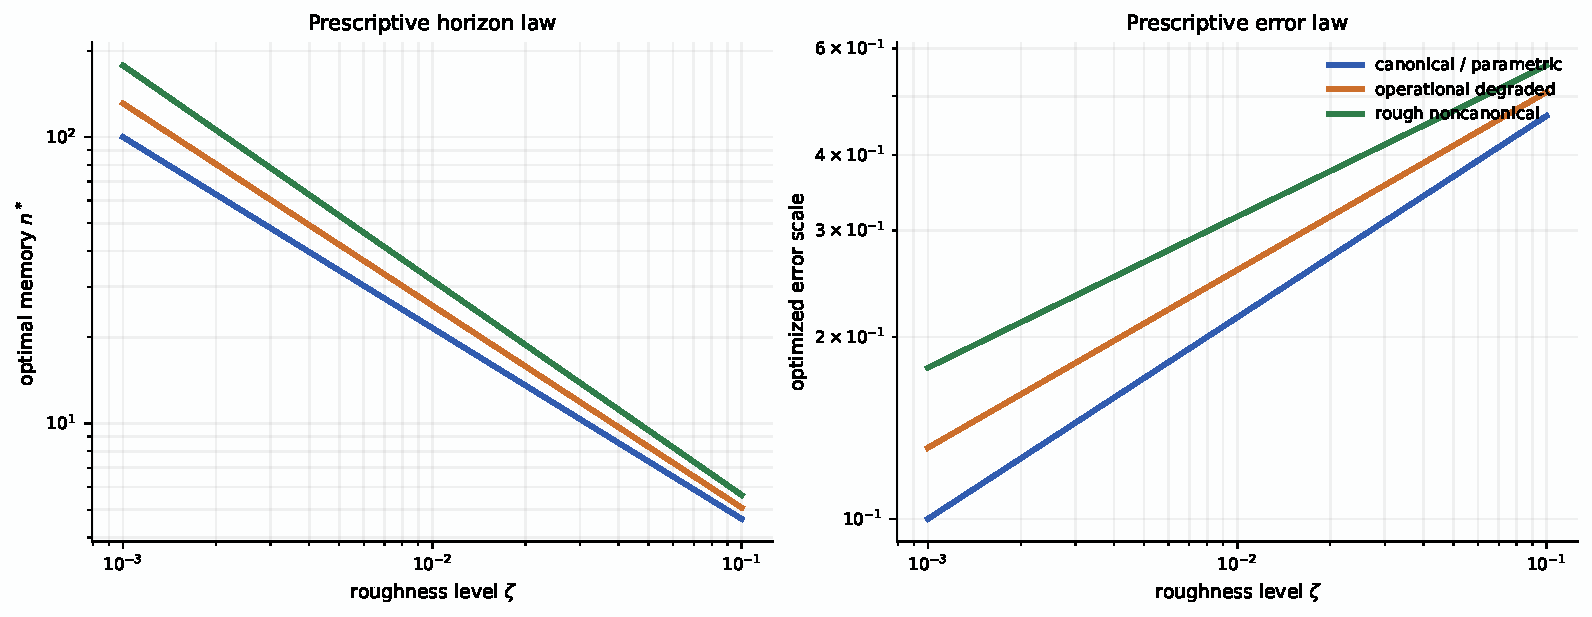
\includegraphics[width=0.92\linewidth]{artifacts/figures/frontier/fig_prescriptive_memory_law.pdf}
\caption{Prescriptive content of the horizon law. The left panel shows the
optimal memory scale $n^*$ and the right panel the optimized error scale for the
$H=1$ slice of the carrier-roughness law, across canonical, degraded
operational, and rough noncanonical carrier regimes. Rougher drift and weaker
carriers both push the optimal policy toward shorter memory and higher residual
error.}
\label{fig:prescriptive_memory_law}
\end{figure}
